\documentclass[unicode,11pt,a4paper,oneside,numbers=endperiod,openany]{article}

\usepackage{float}
\usepackage{enumitem} % \alph*
\usepackage{amsmath,amssymb,amsfonts}
\usepackage{bm}
\usepackage{physics}
\usepackage{graphicx}
\usepackage[makeroom]{cancel}

% \usepackage[utf8]{inputenc}
% \usepackage{wasysym}
% \usepackage{svg}
% \usepackage{fourier}

% \usepackage{minted}
% \usemintedstyle{tango}

\renewcommand{\arraystretch}{1.4}

\title{Scientific Machine Learning \\ Final Project}
\author{Lovnesh Bhardwaj, Laurynas Varnas}
\date{}

\begin{document}
\maketitle

\noindent
Let $\Omega = (0, 1)^2$ be the spatial domain and $I = (0, T]$ a time interval.
We consider the dimensionless monodomain equation, used for simulating
excitable tissues, defined as:

\begin{align*}
	\pdv{u}{t} - \divergence \Sigma \grad u + f(u) & = 0   & \text{in } \Omega \times I,          \\
	\mathbf{n} \cdot \grad u                       & = 0   & \text{on } \partial \Omega \times I, \\
	u                                              & = u_0 & \text{in } \Omega \times \{0\},
\end{align*}

where the reaction term $f$ is given by:

\begin{align*}
	f(u) & = a(u - f_r)(u - f_t)(u - f_d), \\
	a    & = 18.515,                       \\
	f_t  & = 0.2383,                       \\
	f_r  & = 0,                            \\
	f_d  & = 1.
\end{align*}

We assume heterogeneous conductivity across the spatial domain:

\begin{align*}
	\Sigma_h & = 9.5298 \times 10^{-4},                       \\
	\Sigma_d & \in \qty{ 10\Sigma_h, \Sigma_h, 0.1\Sigma_h }.
\end{align*}

The diseased regions are defined as:

\begin{align*}
	\Omega_{d1} & = \qty{ (x, y) \in \Omega \mid (x - 0.3)^2 + (y - 0.7)^2 < 0.1^2 },  \\
	\Omega_{d2} & = \qty{ (x, y) \in \Omega \mid (x - 0.7)^2 + (y - 0.3)^2 < 0.15^2 }, \\
	\Omega_{d3} & = \qty{ (x, y) \in \Omega \mid (x - 0.5)^2 + (y - 0.5)^2 < 0.1^2 }.
\end{align*}

\section{Finite Element Method}


\subsection{IMEX time integration scheme}

We discretize the time interval into steps of size $\Delta t$, and
denote the approximation of $u(x, t_n)$ by $U^n(x)$. The
nonlinear reaction term $f(u)$ is treated explicitly, while the
diffusion term is treated implicitly. The semi-discrete IMEX scheme is:

\begin{align*}
	\frac{U^{n+1} - U^n}{\Delta t} = \divergence \Sigma \grad U^{n+1} - f(U^n).
\end{align*}

Rearranging terms:

\begin{align*}
	U^{n+1} - U^n                                         & = \Delta t\, \divergence \Sigma \grad U^{n+1} - \Delta t\, f(U^n), \\
	U^{n+1} - \Delta t\, \divergence \Sigma \grad U^{n+1} & = U^n - \Delta t\, f(U^n).
\end{align*}

Assuming a spatial discretization with a mesh of size $h$, and denoting
by $A$ the discrete Laplace operator (stiffness matrix), we
obtain the algebraic form:

\begin{align*}
	(\mathbf I - \frac{\Delta t}{h^2} A) U^{n+1} = U^n - \Delta t\, f(U^n).
\end{align*}

We approximate the solution at time $t_n$ by a finite element function:

\begin{align*}
	U^n(x) = \sum_{j=1}^{N} u_j^n \phi_j(x),
\end{align*}

where $\{\phi_j\}_{j=1}^N$ is a basis for the finite element space
$\mathbb{V}_h \subset \mathbb{V}$, and $u_j^n$ are the
coefficients to be computed.


\subsection{Weak formulation at time $t_n$}

Let $v \in \mathbb{V}$. Applying the IMEX time discretization, we multiply the equation by
$v$ and integrate over $\Omega$:

\begin{align*}
	\int_\Omega \frac{U^{n+1} - U^n}{\Delta t} v\,\diffd x +
	\int_\Omega \Sigma \grad U^{n+1} \cdot \grad v\,\diffd x =
	\int_\Omega f(U^n) v\,\diffd x.
\end{align*}

The boundary term vanishes due to the homogeneous Neumann condition:
\[
	\int_{\partial \Omega} (\Sigma \nabla U^{n+1} \cdot \mathbf{n}) v \,\diffd s = 0.
\]

We seek $U^{n+1} \in \mathbb{V}$ such that:

\begin{align*}
	a(U^{n+1}, v) = F(v) \quad \forall v \in \mathbb{V},
\end{align*}

where

\begin{align*}
	a(U^{n+1}, v) & = \int_\Omega \frac{U^{n+1}}{\Delta t} v\,\diffd x
	+ \int_\Omega \Sigma \grad U^{n+1} \cdot \grad v\,\diffd x,                             \\
	F(v)          & = \int_\Omega \left( \frac{U^n}{\Delta t} + f(U^n) \right) v\,\diffd x.
\end{align*}


\subsection{Algebraic formulation of the FEM discretization}

Using the basis functions $\{\phi_j\}$ and the expansion $U^n(x) = \sum_j u_j^n \phi_j(x)$, the weak form becomes a linear system at
each time step:

\begin{align*}
	(\mathbf M + \Delta t\, \mathbf K)\, \mathbf u^{n+1} = \mathbf M\, \mathbf u^n - \Delta t\, \mathbf f(U^n),
\end{align*}

where:

\begin{align*}
	\mathbf M_{ij}   & = \int_\Omega \phi_i(x) \phi_j(x)\,\diffd x \quad                             & \text{(mass matrix)},           \\
	\mathbf K_{ij}   & = \int_\Omega \Sigma(x) \grad \phi_i(x) \cdot \grad \phi_j(x)\,\diffd x \quad & \text{(stiffness matrix)},      \\
	\mathbf f_i(U^n) & = \int_\Omega f(U^n(x)) \phi_i(x)\,\diffd x \quad                             & \text{(nonlinear load vector)}.
\end{align*}

\subsection{Simulation results}

We studied the effect of different diffusivity values in the diseased region,
$\Sigma_d \in \qty{10\Sigma_h, \Sigma_h, 0.1\Sigma_h}$, on the dynamics of wave
propagation. The results show that the activation time increases as $\Sigma_d$
decreases. This is expected, as a lower diffusivity slows down the spread of
excitation through the diseased region. For example, at the finest resolution
($\Delta t = 0.025$, $n_e = 256$), the activation times are approximately 26.18
for $\Sigma_d = 10\Sigma_h$, 27.78 for $\Sigma_d = \Sigma_h$, and 29.23 for
$\Sigma_d = 0.1\Sigma_h$. This trend is consistent across all time steps and
grid resolutions.

We also evaluated the numerical properties of the solution. In particular, we
checked whether the stiffness matrix satisfies the M-matrix condition, which is
associated with stability and monotonicity of the scheme. The results show that
this condition is satisfied only for sufficiently small time steps and fine
meshes. For instance, at $\Delta t = 0.1$, the M-matrix condition fails in most
cases, especially for smaller $\Sigma_d$. At $\Delta t = 0.025$, the condition
is generally satisfied for $\Sigma_d = \Sigma_h$ and $10\Sigma_h$, but not
always for $0.1\Sigma_h$.

Finally, we examined whether the numerical solution stays within the physically
meaningful range $u \in [0, 1]$. Again, this requirement is met only when the
mesh and time step are fine enough. Coarse discretizations tend to produce
values outside the expected bounds, particularly when $\Sigma_d$ is small. This
suggests that smaller diffusivity increases the stiffness of the problem,
requiring more careful numerical treatment to ensure accurate results.

\begin{table}[H]
	\centering
	\caption{Results of the simulation for $\Sigma_d = 10\Sigma_h$.}
	\begin{tabular}{l|r|ccc}
		$\Delta t$ & $n_e$ & Activation time & M-matrix? & $u \in [0, 1]$ \\
		\hline
		0.1        & 64    & 28.60           & true      & false          \\
		0.1        & 128   & 29.10           & true      & false          \\
		0.1        & 256   & 29.20           & true      & false          \\
		0.05       & 64    & 26.60           & false     & false          \\
		0.05       & 128   & 27.15           & true      & true           \\
		0.05       & 256   & 27.20           & true      & true           \\
		0.025      & 64    & 25.60           & false     & false          \\
		0.025      & 128   & 26.10           & true      & true           \\
		0.025      & 256   & 26.175          & true      & true           \\
	\end{tabular}
\end{table}

\begin{table}[H]
	\centering
	\caption{Results of the simulation for $\Sigma_d = \Sigma_h$.}
	\begin{tabular}{l|r|ccc}
		$\Delta t$ & $n_e$ & Activation time & M-matrix? & $u \in [0, 1]$ \\
		\hline
		0.1        & 64    & 30.20           & true      & false          \\
		0.1        & 128   & 30.90           & true      & false          \\
		0.1        & 256   & 31.00           & true      & false          \\
		0.05       & 64    & 28.10           & false     & false          \\
		0.05       & 128   & 28.80           & true      & true           \\
		0.05       & 256   & 28.90           & true      & true           \\
		0.025      & 64    & 27.025          & false     & false          \\
		0.025      & 128   & 27.70           & true      & true           \\
		0.025      & 256   & 27.775          & true      & true           \\
	\end{tabular}
\end{table}

\begin{table}[H]
	\centering
	\caption{Results of the simulation for $\Sigma_d = 0.1\Sigma_h$.}
	\begin{tabular}{l|r|ccc}
		$\Delta t$ & $n_e$ & Activation time & M-matrix? & $u \in [0, 1]$ \\
		\hline
		0.1        & 64    & 31.70           & false     & false          \\
		0.1        & 128   & 32.50           & false     & false          \\
		0.1        & 256   & 32.60           & true      & false          \\
		0.05       & 64    & 29.55           & false     & false          \\
		0.05       & 128   & 30.25           & false     & false          \\
		0.05       & 256   & 30.40           & false     & true           \\
		0.025      & 64    & 28.40           & false     & false          \\
		0.025      & 128   & 29.075          & false     & false          \\
		0.025      & 256   & 29.225          & false     & true           \\
	\end{tabular}
\end{table}

Overall, the results confirm that lower diffusivity in the diseased region
significantly slows wave propagation and makes the numerical problem more
challenging. Finer meshes and smaller time steps are necessary to maintain both
accuracy and physical realism.

\begin{figure}[H]
	\centering
	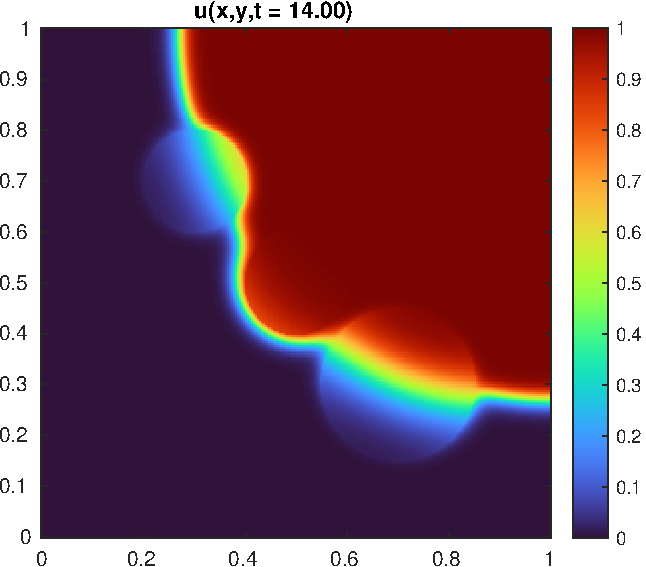
\includegraphics[width=0.45\textwidth]{figs/S10.pdf}
	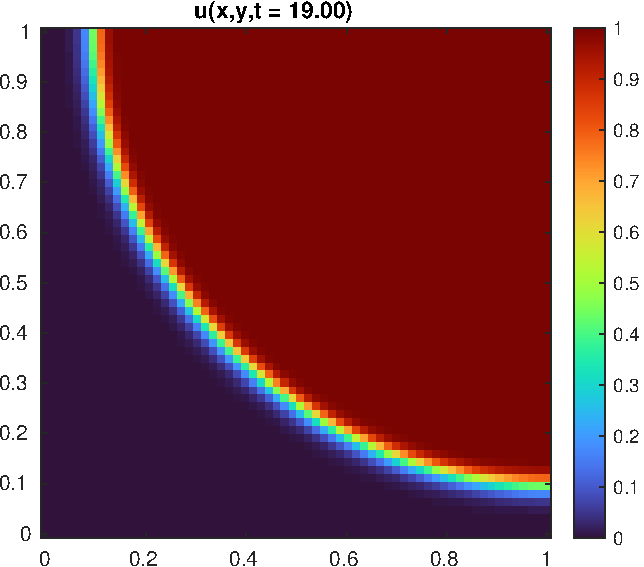
\includegraphics[width=0.45\textwidth]{figs/S1.pdf}
	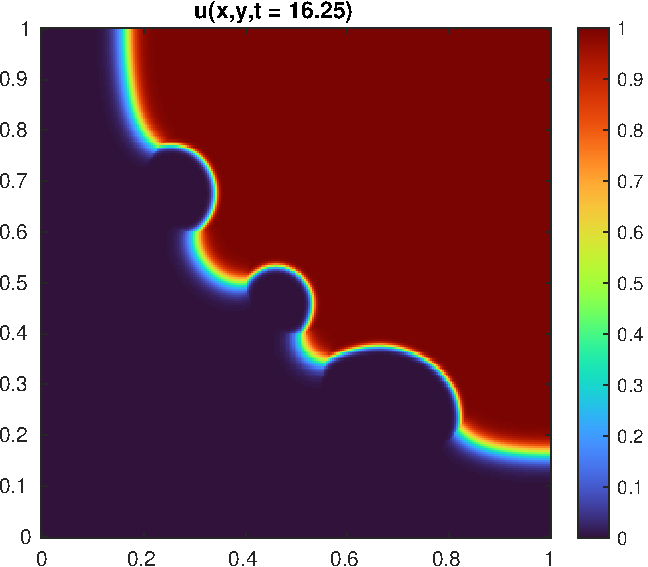
\includegraphics[width=0.45\textwidth]{figs/S01.pdf}
	\caption{Snapshots of the simulation over diseased regions for $\Sigma_d \in \qty{10\Sigma_h, \Sigma_h, 0.1\Sigma_h}$.}
\end{figure}

\nocite{*}
\bibliographystyle{abbrv}
\bibliography{biblio}

\end{document}


% vi:nowrap
